% Auto-generated figure includes for main.tex
% Run: python paper/generate_figures.py

\begin{figure*}[t]
    \centering
    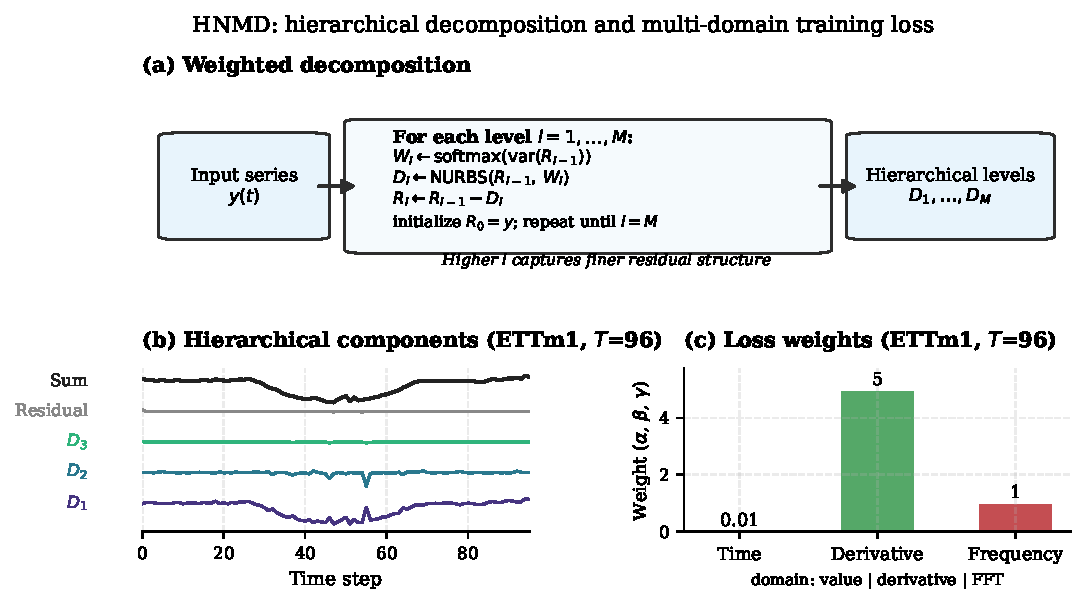
\includegraphics[width=\textwidth]{figures/fig1_method_overview.pdf}
    \caption{Overview of HNMD. \textbf{(a)} Variance-conditioned NURBS decomposition of the residual at each level.
    \textbf{(b)} Hierarchical components from NURBS decomposition of an ETTm1 test window ($T{=}96$).
    \textbf{(c)} Tuned $\alpha$, $\beta$, $\gamma$ for ETTm1 / MLP / $T{=}96$ (Table~\ref{tab:hyper}).}
    \label{fig:method}
\end{figure*}

\begin{figure*}[t]
    \centering
    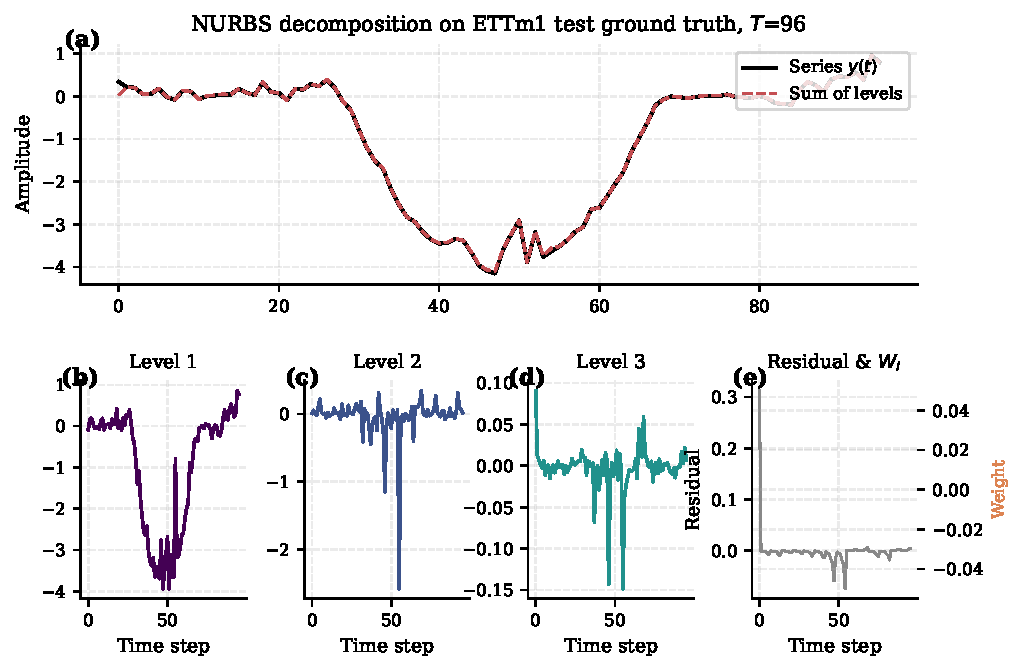
\includegraphics[width=\textwidth]{figures/fig2_decomposition.pdf}
    \caption{NURBS decomposition of an ETTm1 test ground-truth window ($T{=}96$).
    \textbf{(a)} Original series and sum of fitted levels. \textbf{(b--d)} Individual levels. \textbf{(e)} Final residual and regional variance weights.}
    \label{fig:decomposition}
\end{figure*}

\begin{figure}[t]
    \centering
    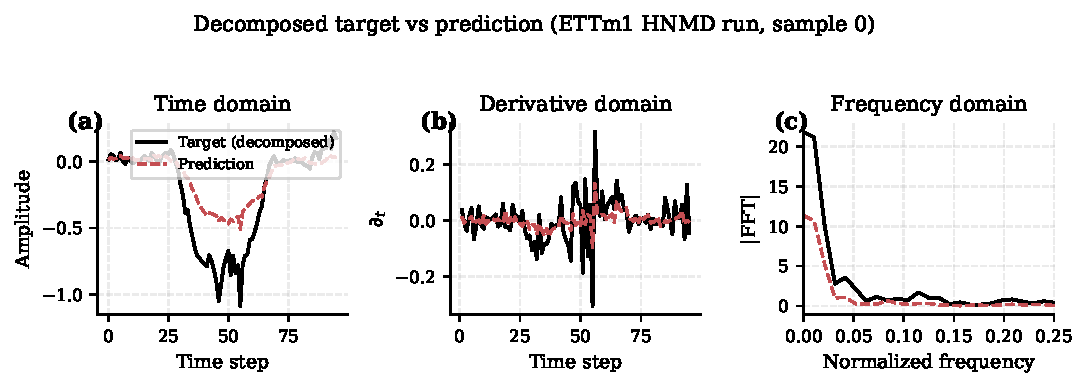
\includegraphics[width=\columnwidth]{figures/fig3_multidomain.pdf}
    \caption{Decomposed target vs.\ HNMD prediction (ETTm1, $T{=}96$) in time, derivative, and frequency domains.}
    \label{fig:multidomain}
\end{figure}

\begin{figure}[t]
    \centering
    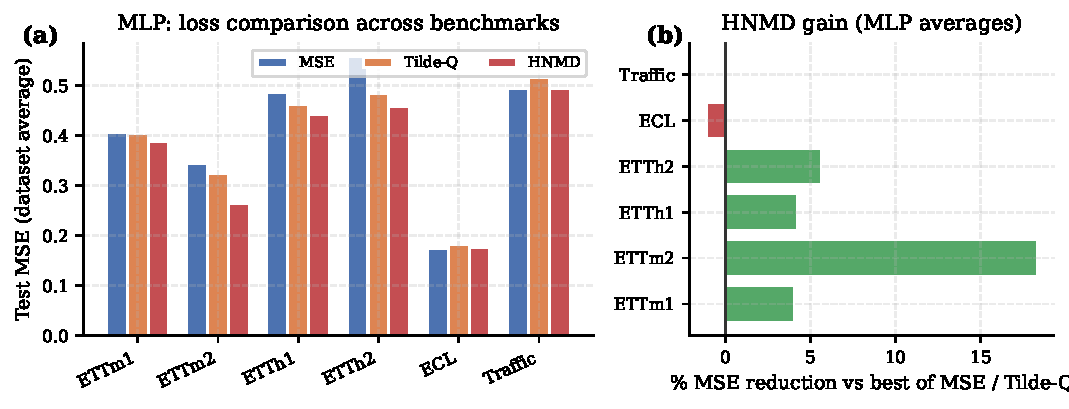
\includegraphics[width=\columnwidth]{figures/fig4_mlp_results.pdf}
    \caption{MLP test MSE (mean over horizons) from \texttt{./results/}. \textbf{(a)} MSE, Tilde-Q, and HNMD. \textbf{(b)} Percent improvement of HNMD over the better of MSE/Tilde-Q where both exist.}
    \label{fig:mlp-results}
\end{figure}

\begin{figure*}[t]
    \centering
    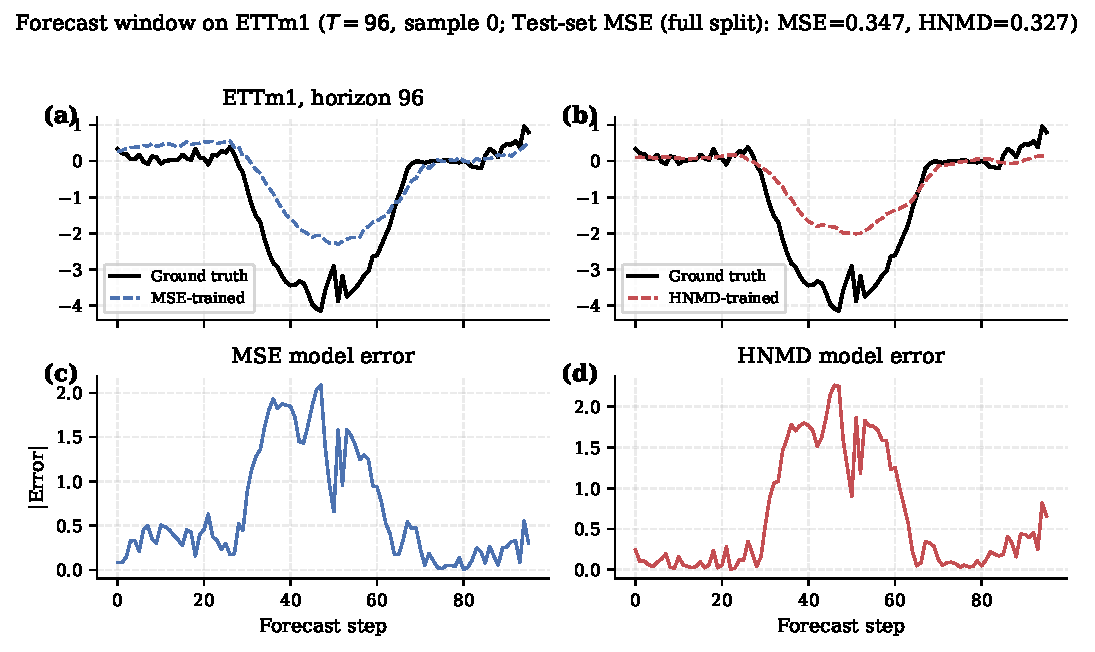
\includegraphics[width=\textwidth]{figures/fig5_forecast_comparison.pdf}
    \caption{Forecast window from saved \texttt{pred.npy}/\texttt{true.npy} (ETTm1, $T{=}96$). \textbf{(a,b)} MSE- vs HNMD-trained MLP. \textbf{(c,d)} Absolute errors. Suptitle gives full test-split MSE.}
    \label{fig:forecasts}
\end{figure}

\begin{figure}[t]
    \centering
    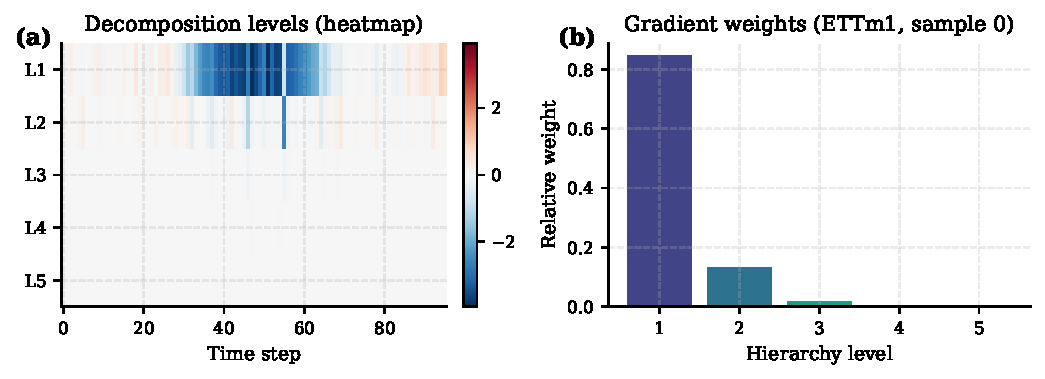
\includegraphics[width=\columnwidth]{figures/fig6_level_importance.pdf}
    \caption{NURBS levels (heatmap) and per-level gradient weights from MSSD on an ETTm1 test window ($T{=}96$).}
    \label{fig:level-importance}
\end{figure}
